% Martin Rodriguez Jr.
% SID: 811958765


%Anything following a % sign is a comment.
%Please use the comments to help you understand the code below.

%%%%%%%%%%%% Quick Notes %%%%%%%%%%%%%%%%%%%%%%

% \textit{} ==> italicises words or phrases
% \textbf{} ==> bolds words or phrases
% \\ ==> creates a new line
% \S ==> creates section section symbol, fancy double s thing
% \renewcommand{\baselinest8retch}{2} ==> double spaces the document

%%%%%%%%%%%%%%%%%%%%%%%%%%%%%%%%%%%%%%%%
\documentclass[12pt]{article}

%LOAD VARIOUS PACKAGES
\usepackage{setspace}
\usepackage{caption}
\usepackage{subcaption}
\usepackage{graphics, latexsym, multicol}		%
\usepackage{graphicx}
\usepackage{lscape}

\usepackage{amsmath, amsfonts, amsthm, amssymb}		%Math packages provided by American Math Society (AMS)
\usepackage{thmtools}

\usepackage{xcolor}							%Extended color package: provides colors for text enhancement
%\usepackage[margin = 1.00in, top = 1in, bottom = 1in, nohead] {geometry}
\usepackage{boxedminipage}					%allows use of boxed minipages
\usepackage{enumitem}
\setlist{itemsep=-6pt}

\usepackage[english]{babel}
\usepackage{xcolor} % Required for specifying custom colors
\usepackage{fix-cm} % Allows increasing the font size of specific fonts beyond LaTeX default specifications

\usepackage{longtable}

%MATH CHARACTER COMMANDS: Short hand for commands
\def\N{\mathbb{N}}		 				%Natual Bold Face: \N is now the command for the Natural Numbers
\def\Q{\mathbb{Q}} 						%Rational Bold Face: \R
\def\R{\mathbb{R}} 						%Real Bold Face
\def\Z{\mathbb{Z}} 						%Integers Bold Face
\def\C{\mathbb{C}} 						%Complex Bold Face
\def\eps{\varepsilon}                                               % Defines \varepsilon to \eps
\renewcommand{\qedsymbol}{$\blacksquare$} % QED symbol

\def\L{\mathcal{L}}

\def\flecha{$\rightarrow \,$}
\def\fflecha{$\Rightarrow \,$}

%Solution template with little sideways triangle
\declaretheoremstyle[
spaceabove=6pt, spacebelow=6pt,
headfont=\normalfont\bfseries,
notefont=\mdseries, notebraces={(}{)},
bodyfont=\normalfont,
postheadspace=1em,
numberwithin=section
]{exstyle}
\declaretheoremstyle[
spaceabove=6pt, spacebelow=6pt,
headfont=\normalfont\bfseries,
notefont=\mdseries, notebraces={(}{)},
bodyfont=\normalfont,
postheadspace=1em,
headpunct={},
qed=$\blacktriangleleft$,
numbered=no
]{solstyle}
\declaretheorem[style=exstyle]{example}
\declaretheorem[style=solstyle]{solution}

%\newenvironment{solution}
%  {\begin{proof}[Solution]}
%  {\end{proof}}
%
%



\usepackage{hyperref}
\usepackage{listings}



\begin{document}

\begin{center}
	{\LARGE Linear Advection and Diffusion} \\[10pt] 
	AMS 209: Foundations of Scientific Computing\\
	Fall 2017 \\
	{Martin Rodriguez} \\
\end{center}

\begin{abstract}
	The goal of this project to use model a one-dimensional advection and diffusion equation numerically. For diffusion we used a centered spatial discretization and forward time. In the case of advection, we continue to use forward time and use both an backward space also called upwind and a centered difference. The code is tested on a grid size of $N= 32$ and $N=128$ for the diffusion, advection, and the advection-diffusion case. The upwind method provides the best solution for the advection partial differential equation (PDE) and the center finite difference method solutions explodes eventually. However, when viscosity is added then the center method resolves the PDE. 
\end{abstract}

\newpage

\section{Methods}

	There were two parts to the project. We needed to implement the PDE solver in Fortran and a Python scheduler. The Fortran implementation solves
	\begin{align}
		u_t + au_x = \kappa u_{xx},
	\end{align}
	with two subcases where $a = 0$ and $\kappa = 0$. In the following sections we will describe the discretization methods and the modules implementation.

	\subsection{Discretization}
		When solving the diffusion equation then we discretization using
		\begin{align}
			u_i^{n+1} = u_i^n + \kappa \frac{\Delta t}{\Delta x^2} ( u_{i+1}^n - 2u_i^n + u_{i-1}^n ), 
		\end{align}
		and we need to satisfy the CFL condition
		\begin{align*}
			\kappa \Delta t \leq \frac{\Delta x^2}{2}.
		\end{align*}
		The diffusion equation uses the initial condition
		\begin{align*}
			u_0 = \begin{cases}0 , & x\in [0,1) \\ 100 , & x = 1 \end{cases}
		\end{align*}
		The diffusion solver is implemented \texttt{pde\_solver\_module.F90} in the function \texttt{diffuse\_update()}.
		
		When solving the advection PDE then we use the upwind discretization 
		\begin{align}
			u_i^{n+1} = u_i^n - \frac{a\Delta t}{\Delta x} (u_i^n - u_{i-1}^n)
		\end{align}
		and the centered discretization shown below
		\begin{align}
			u_i^{n+1} = u_i^n - \frac{a\Delta t}{2\Delta x} (u_{i+1}^n - u_{i-1}^n).
		\end{align}
		The advection method needs to satisfy the CFL condition
		\begin{align}
			|a| \Delta \leq \Delta x.
		\end{align}
		This portion is implemented in the \texttt{pde\_solver\_module.F90} in the function \texttt{advect\_update()}.

		
		\subsection{Fortran Modules}
		In this code we implemented a total of four modules and the driver. The modules are the following:
		\begin{itemize}
			\item \texttt{advection\_diffusion.F90}: This file is driver of the entire code. All of the subroutines are called from here and results are are saved to a text file. 
			\item \texttt{setup\_module.F90}: This module calls the file \texttt{pde.init} and sets up all of the runtime parameters.
			\item \texttt{initialize\_module.F90}: This modules includes the subroutines \texttt{grid\_init()}, \texttt{diffuse\_init(uold)}, \texttt{advect\_init(x,uold)}, and the \texttt{simulation\_init(x,uold)}. This module serves to initialize the grid and the initial conditions for the diffusion equation or the advection or the advection-diffusion equation.
			\item \texttt{pde\_solver\_module.F90}: This module includes all the necessary pieces for solving the PDE. It includes \texttt{cfl()}, \texttt{bc(unew)}, \texttt{diffuse\_update(uold,unew)}, \texttt{advect\_update(uold,unew)}, \texttt{check\_error(uold,unew)}, and \linebreak\texttt{compute\_timestep(t,frameNumber,writeOutput)}. The \texttt{compute\_timestep} module computes the time step but checks whether the time step is small enough to write the data at every tenth of a second. The input \texttt{frameNumber} counts the number of frames that have been saved to a text file. 
		\end{itemize}


\section{Results and Discussion}
	\begin{enumerate}[label=(\alph*)]
		\item The Figures \ref{fig:diff1} through \ref{fig:diff4} show the solution to diffusion equation as it reaches steady state with $N = 32$. The $t_{max} = 0.7$. The figures \ref{fig:diff5} through \ref{fig:diff8} show the diffusion equation with $N=128$.
		\begin{figure}[htb]
		\centering
		\begin{minipage}[c]{0.48\textwidth}
			\centering
			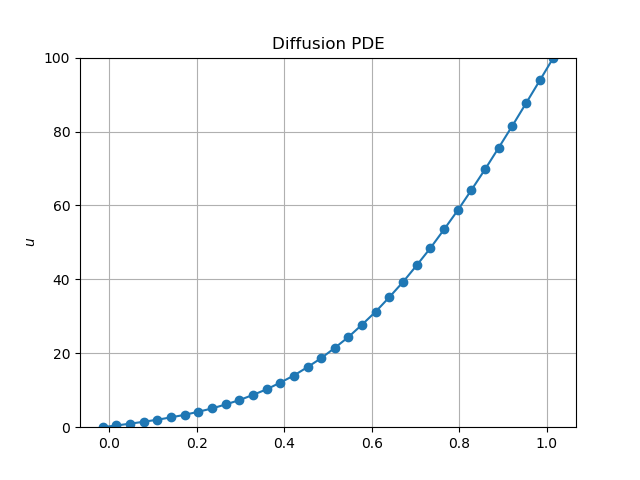
\includegraphics[width=0.7\linewidth]{./PDE/figures/diffusion_32_upwind/result_diffusion_32_upwind_1.png}
			\caption{This is diffusion at 0.2$t_{max}$.}
			\label{fig:diff1}
		\end{minipage}
		\hspace{0.1in}
		\begin{minipage}[c]{0.48\textwidth}
			\centering
			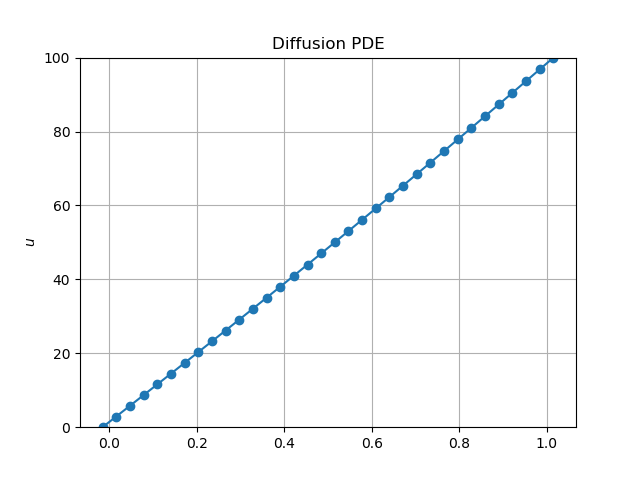
\includegraphics[width=0.7\linewidth]{./PDE/figures/diffusion_32_upwind/result_diffusion_32_upwind_5.png}
			\caption{This is diffusion at 0.5$t_{max}$.}
			\label{fig:diff2}
		\end{minipage}
		\newline
		\vspace{-0.2in}
	\end{figure}
	\newpage
	\begin{figure}[htb]
		\centering
		\begin{minipage}[c]{0.48\textwidth}
			\centering
			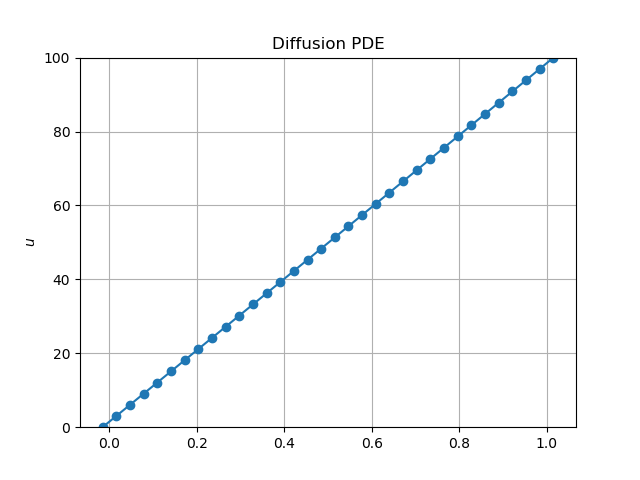
\includegraphics[width=0.7\linewidth]{./PDE/figures/diffusion_32_upwind/result_diffusion_32_upwind_8.png}
			\caption{This is diffusion at 0.8$t_{max}$.}
			\label{fig:diff3}
		\end{minipage}
		\hspace{0.1in}
		\begin{minipage}[c]{0.48\textwidth}
			\centering
			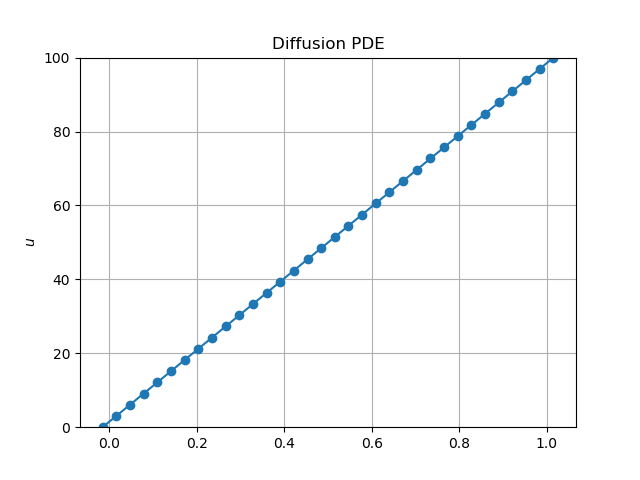
\includegraphics[width=0.7\linewidth]{./PDE/figures/diffusion_32_upwind/result_diffusion_32_upwind_10.png}
			\caption{This is diffusion at $t_{max}$.}
			\label{fig:diff4}
		\end{minipage}
		\newline
		\vspace{-0.2in}
	\end{figure}
		
		
	\begin{figure}[htb]
		\centering
		\begin{minipage}[c]{0.48\textwidth}
			\centering
			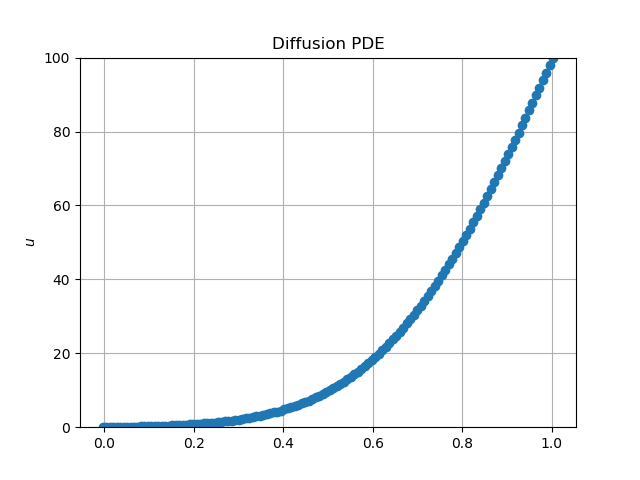
\includegraphics[width=0.7\linewidth]{./PDE/figures/diffusion_128_upwind/result_diffusion_128_upwind_1.png}
			\caption{This is diffusion at 0.2$t_{max}$.}
			\label{fig:diff5}
		\end{minipage}
		\hspace{0.1in}
		\begin{minipage}[c]{0.48\textwidth}
			\centering
			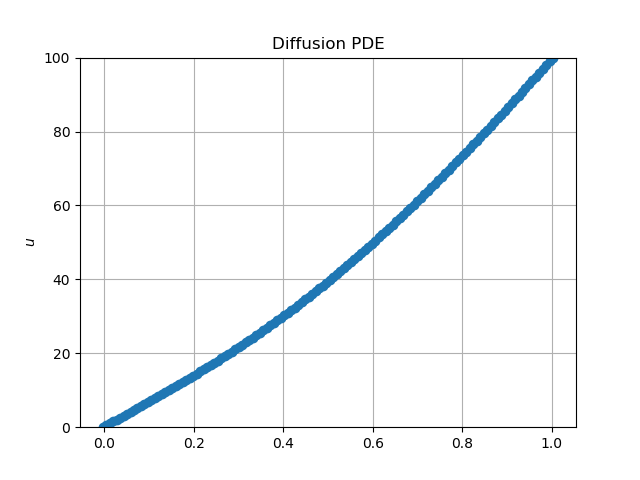
\includegraphics[width=0.7\linewidth]{./PDE/figures/diffusion_128_upwind/result_diffusion_128_upwind_4.png}
			\caption{This is diffusion at 0.5$t_{max}$.}
			\label{fig:diff6}
		\end{minipage}
		\newline
		\vspace{-0.2in}
	\end{figure}
	\begin{figure}[htb]
		\centering
		\begin{minipage}[c]{0.48\textwidth}
			\centering
			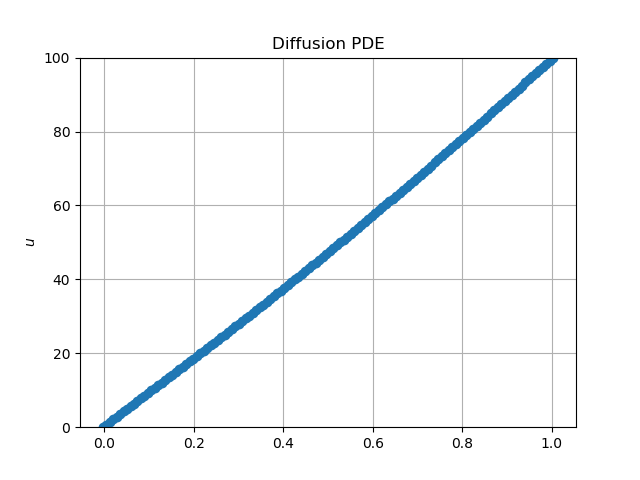
\includegraphics[width=0.7\linewidth]{./PDE/figures/diffusion_128_upwind/result_diffusion_128_upwind_7.png}
			\caption{This is diffusion at 0.8$t_{max}$.}
			\label{fig:diff5}
		\end{minipage}
		\hspace{0.1in}
		\begin{minipage}[c]{0.48\textwidth}
			\centering
			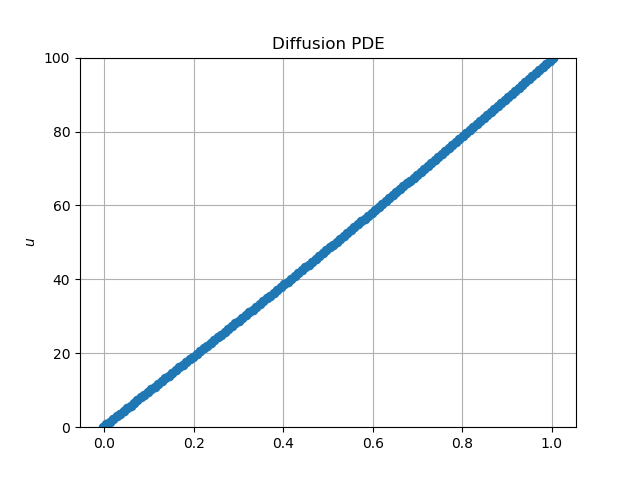
\includegraphics[width=0.7\linewidth]{./PDE/figures/diffusion_128_upwind/result_diffusion_128_upwind_8.png}
			\caption{This is diffusion at $t_{max}$.}
			\label{fig:diff8}
		\end{minipage}
		\newline
		\vspace{-0.2in}
	\end{figure}
	
	\vspace{0.25in}
	
	\item The max time for the case $N = 32$ is $t_{max} = 0.70$ while for $N=128$ the $t_{max} =0.41$. I believe that the finer grid increases the accuracy and thus reaching a steady state much faster. 
	
	\item If the $\Delta t_{diff}$ does not satisfy the CFL condition then numerical method will unstable and not solve the equation. 
	
	\item There is discrepancy in the max time found for both grids. The max time for the coarser grid is 0.70 while for the finer grid it was 0.41. 
	
	\item In order to see one period of the advection PDE then we need to run the time to $t_{max} = 1$.
	
	\item In the following we show the solution of the Advective PDE in with $N=32$ and $N=128$ with both the discretization types. Figures \ref{fig:ad1} and \ref{fig:ad2} show the solution using the upwind method while Figures \ref{fig:ad3} and \ref{fig:ad4}.

	\begin{figure}[htb]
		\centering
		\begin{minipage}[c]{0.48\textwidth}
			\centering
			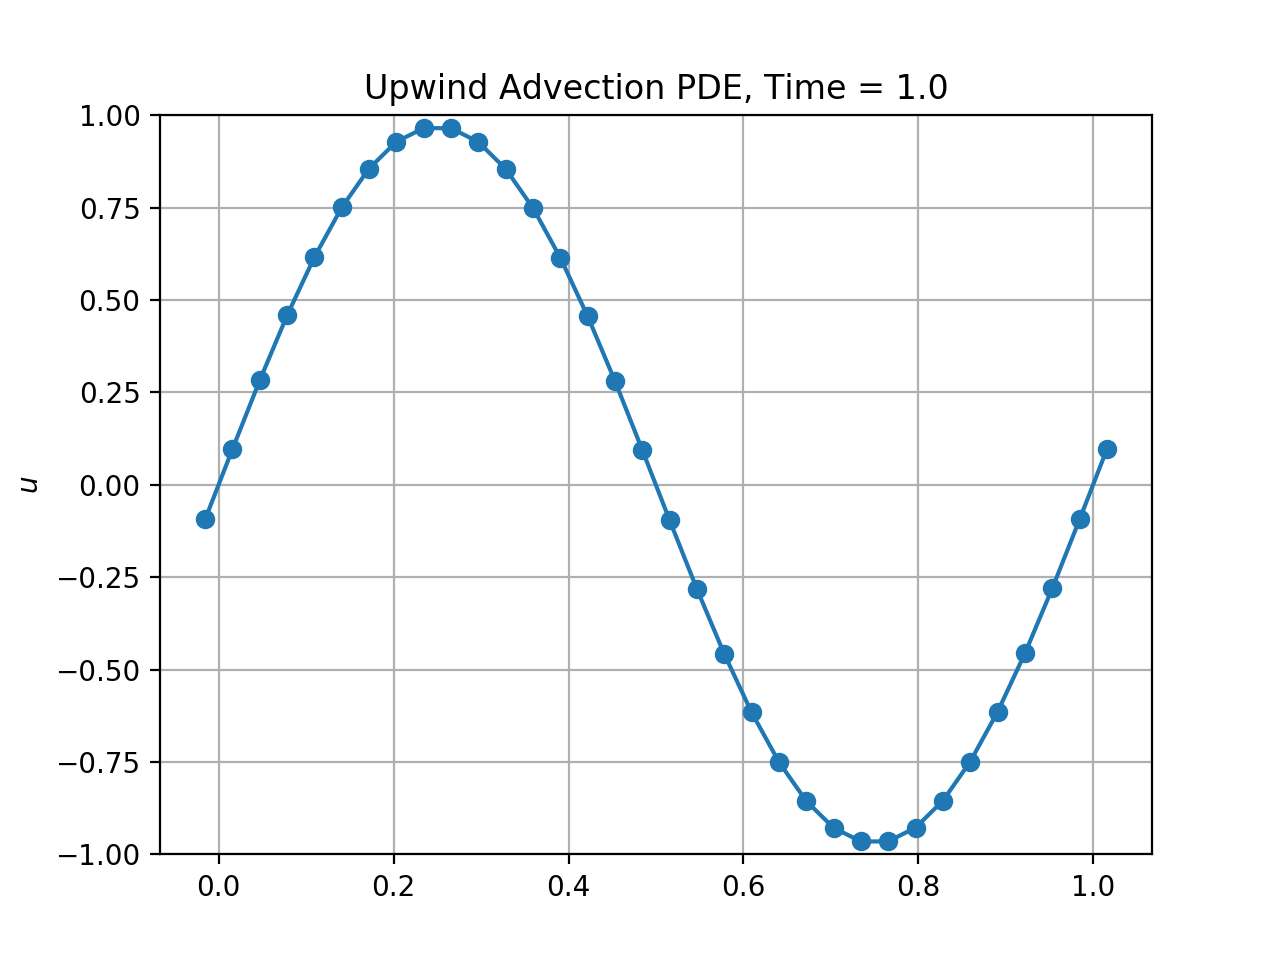
\includegraphics[width=0.7\linewidth]{./PDE/figures/advection_32_upwind/result_advection_32_upwind_1.png}
			\caption{This is advection at $t_{max} = 1$.}
			\label{fig:ad1}
		\end{minipage}
		\hspace{0.1in}
		\begin{minipage}[c]{0.48\textwidth}
			\centering
			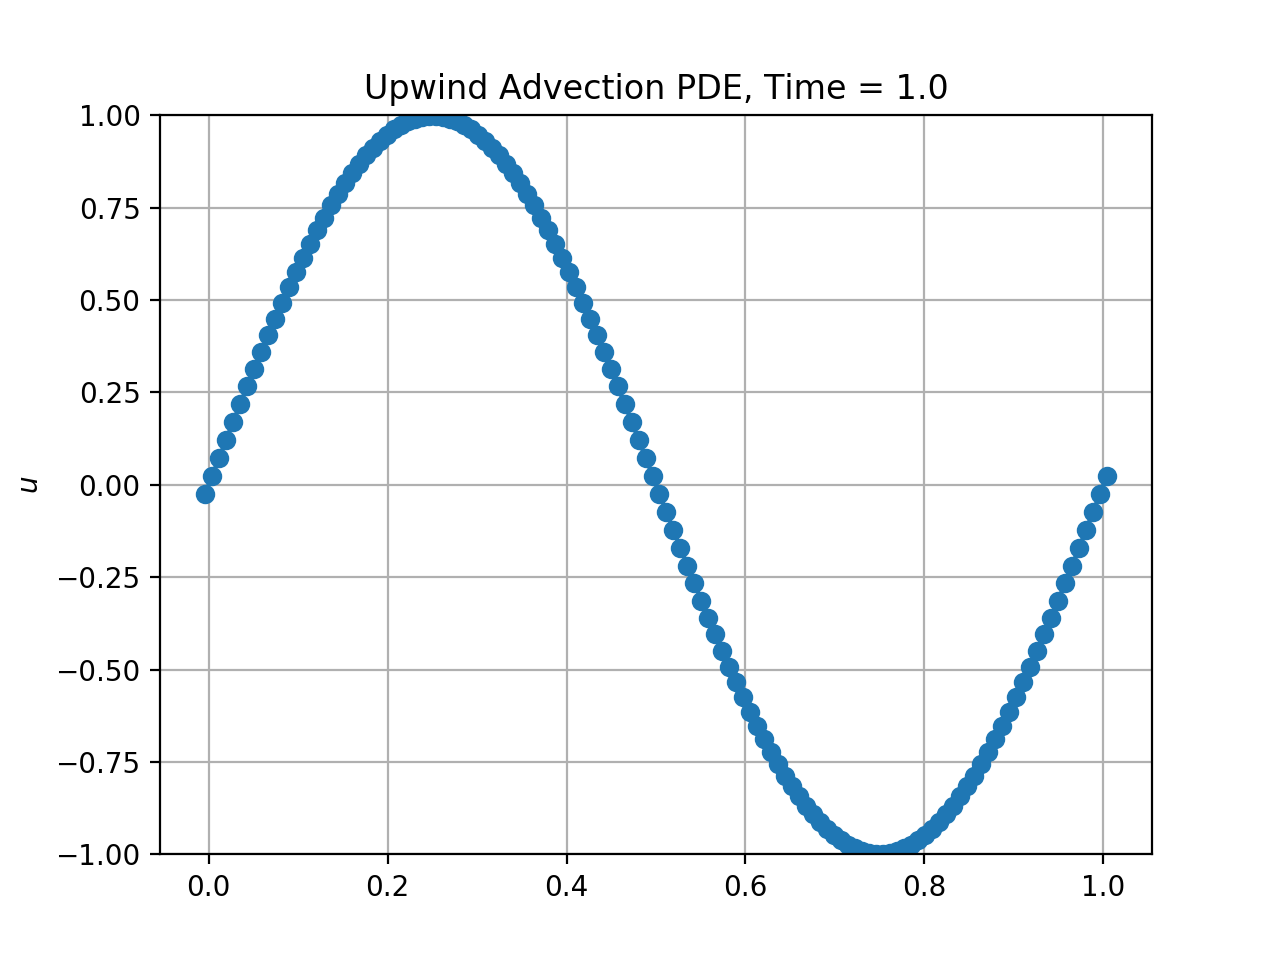
\includegraphics[width=0.7\linewidth]{./PDE/figures/advection_128_upwind/result_advection_128_upwind_1.png}
			\caption{This is advection at $t_{max} = 1$.}
			\label{fig:ad2}
		\end{minipage}
		\newline
		\vspace{-0.2in}
	\end{figure}
		\begin{figure}[htb]
		\centering
		\begin{minipage}[c]{0.48\textwidth}
			\centering
			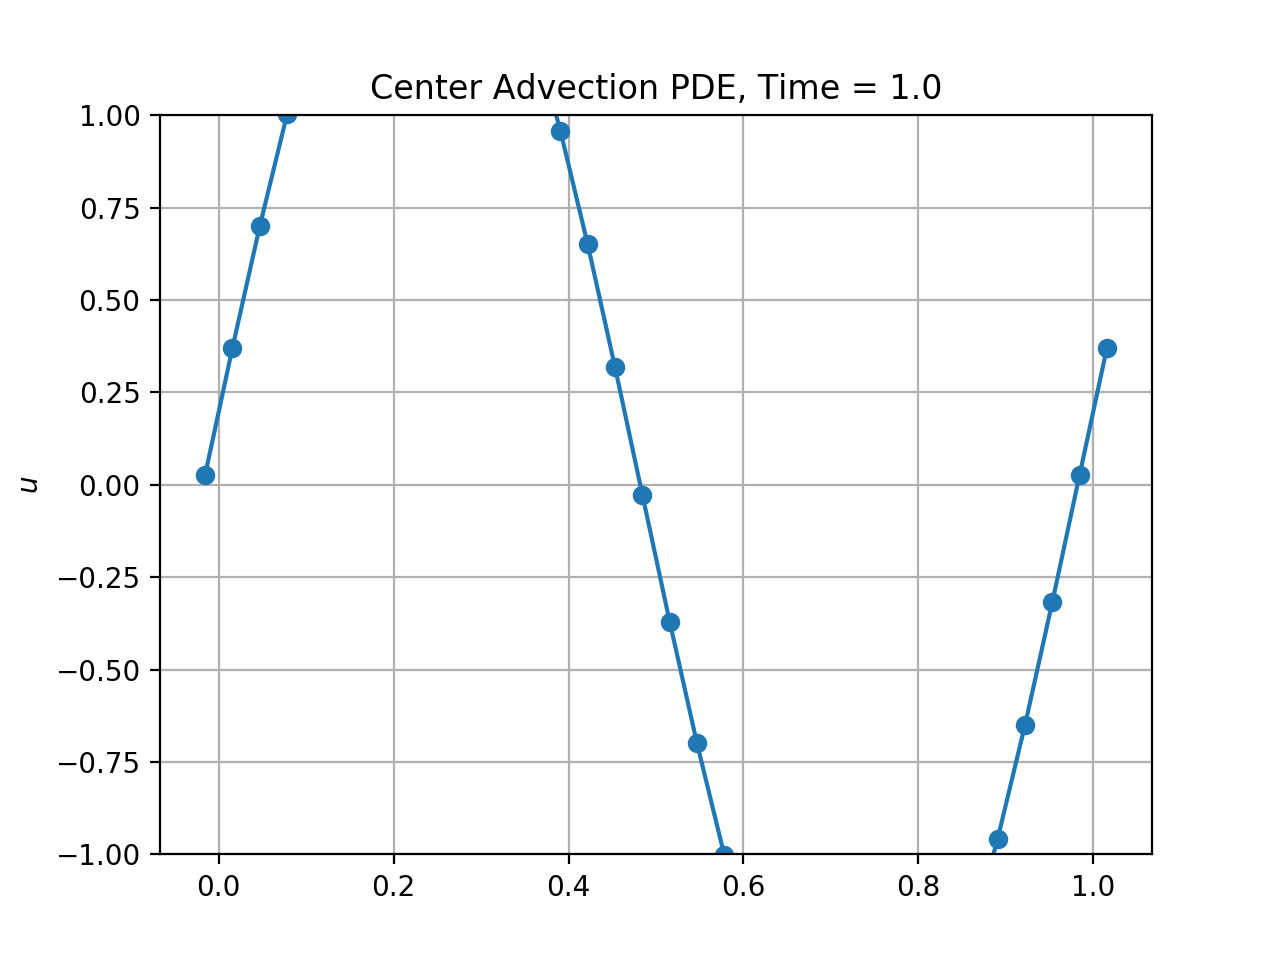
\includegraphics[width=0.7\linewidth]{./PDE/figures/advection_32_center/result_advection_32_center_1.png}
			\caption{This is diffusion at $t_{max} = 1$.}
			\label{fig:ad3}
		\end{minipage}
		\hspace{0.1in}
		\begin{minipage}[c]{0.48\textwidth}
			\centering
			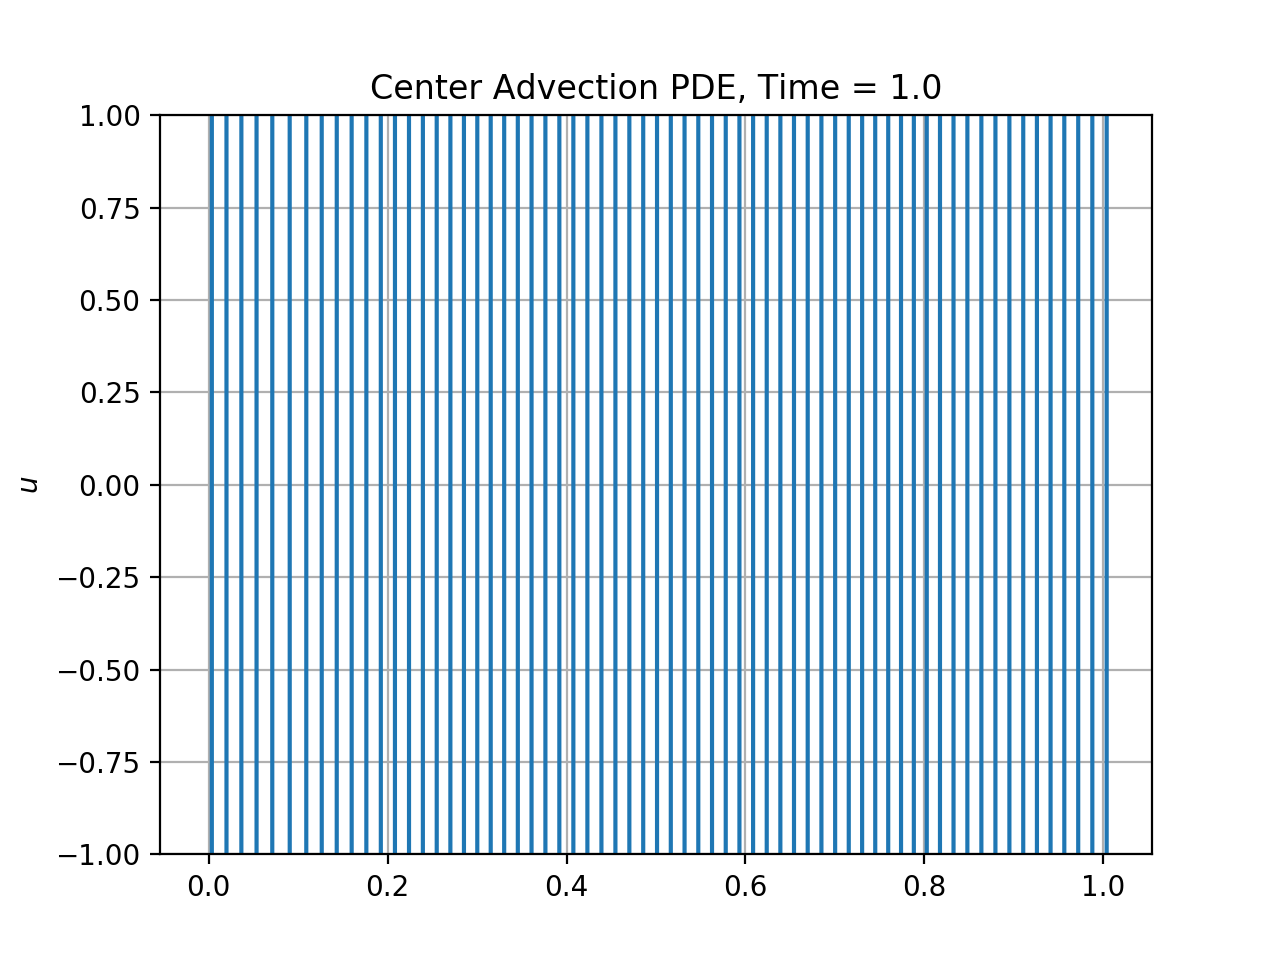
\includegraphics[width=0.7\linewidth]{./PDE/figures/advection_128_center/result_advection_128_center_1.png}
			\caption{This is advection at $t_{max} = 1$.}
			\label{fig:ad4}
		\end{minipage}
		\newline
		\vspace{-0.2in}
	\end{figure}
	
	
	\item As we saw from the previous figures the best method is the upwind discretization. So now we let $Ca = 0.9$ and $Ca = 1.2$ as shown in Figures \ref{fig:calow} and \ref{fig:cahigh}. We can see that for $Ca = 0.9$ the system loses energy. In contrast, when $Ca = 1.2$ then the system gains energy. 
	\newpage
	\begin{figure}[htb]
		\centering
		\begin{minipage}[c]{0.48\textwidth}
			\centering
			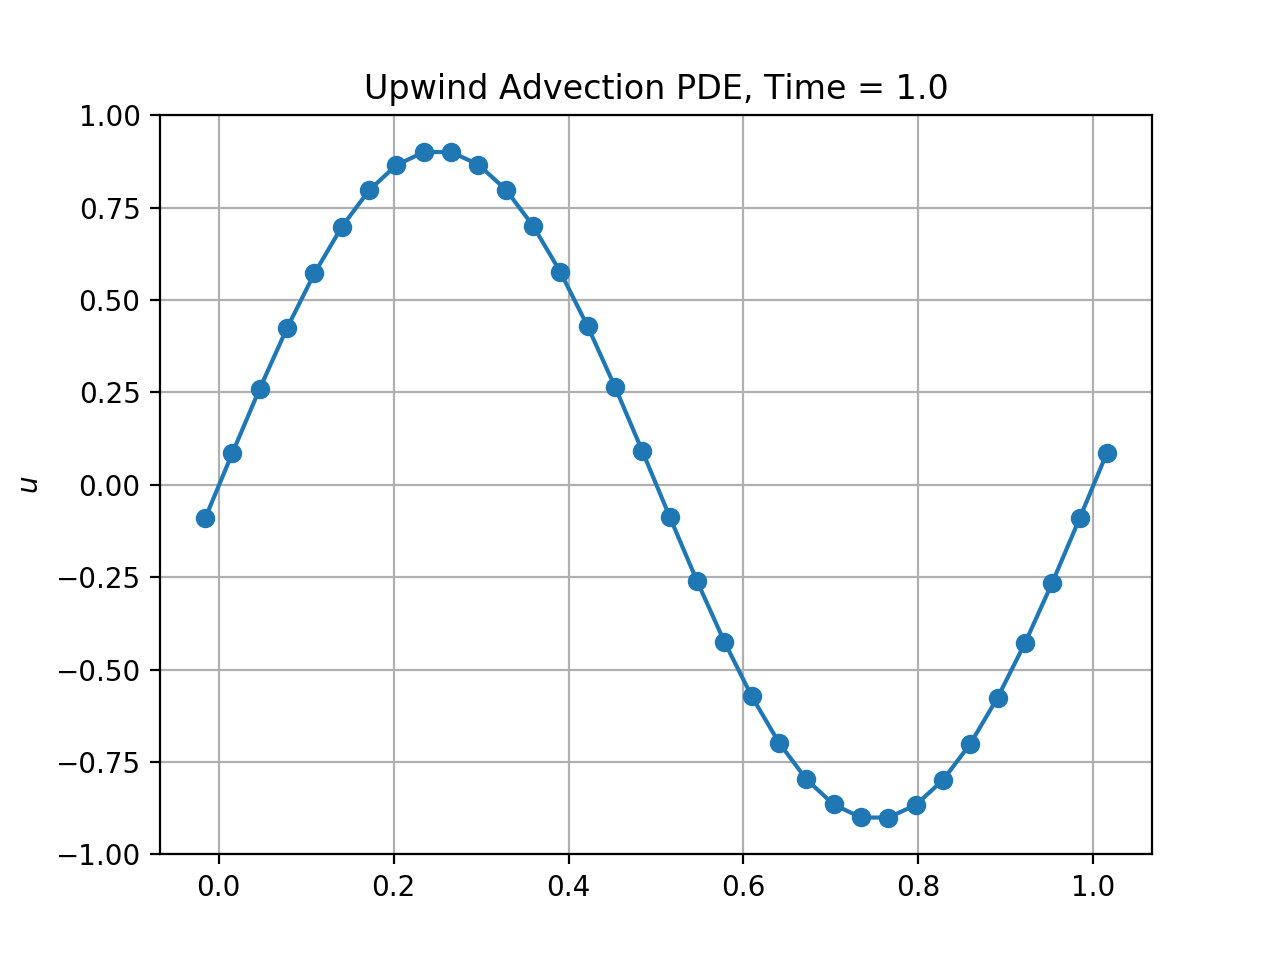
\includegraphics[width=0.7\linewidth]{./PDE/figures/plotsforg/result_advection_32_upwind_1_lowCa.png}
			\caption{This has a CFL constant of $Ca = 0.9$.}
			\label{fig:calow}
		\end{minipage}
		\hspace{0.1in}
		\begin{minipage}[c]{0.48\textwidth}
			\centering
			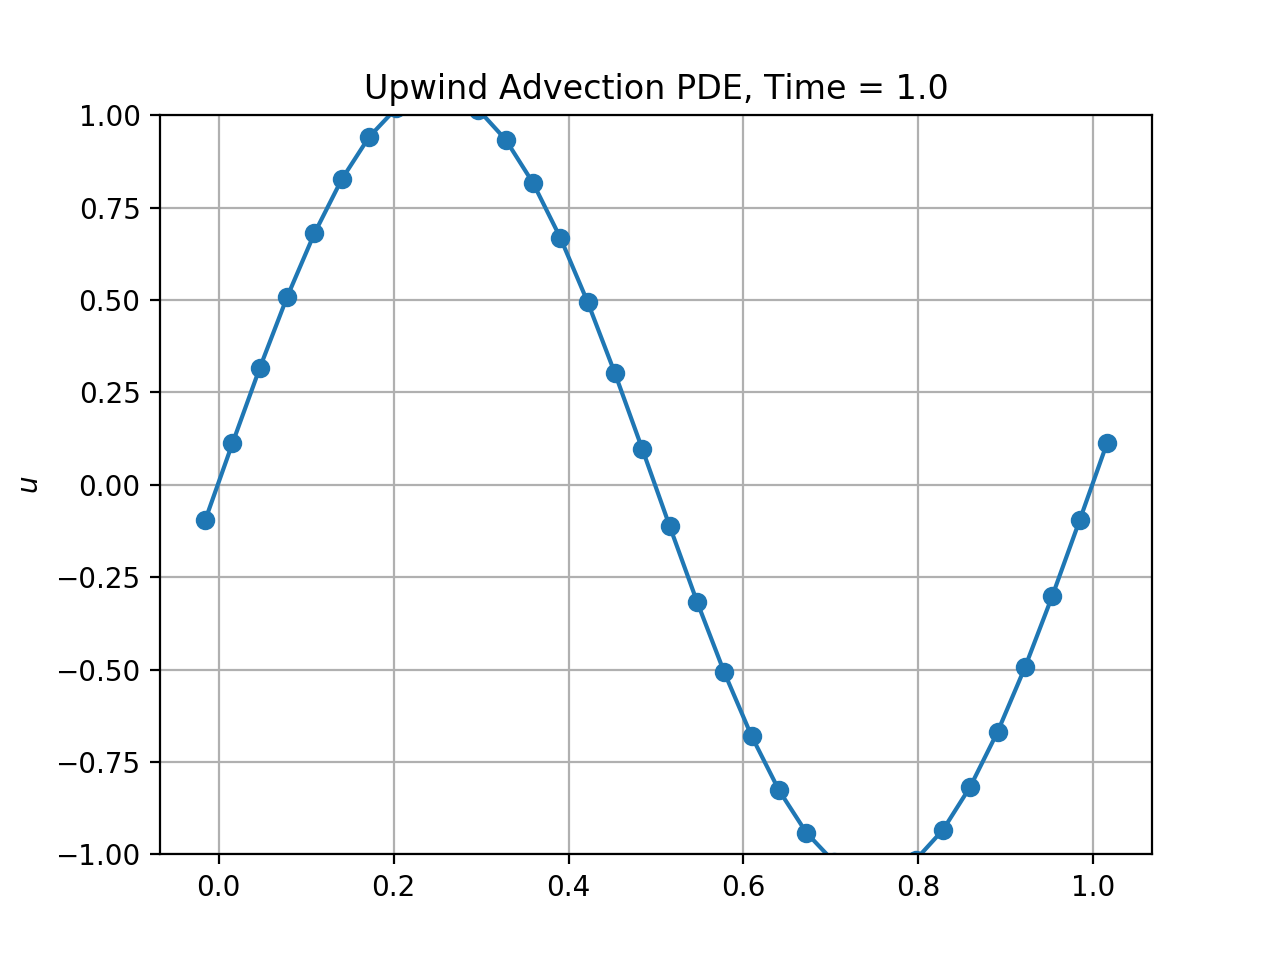
\includegraphics[width=0.7\linewidth]{./PDE/figures/plotsforg/result_advection_32_upwind_1_highCa.png}
			\caption{This has a CFL constant of $Ca = 1.2$.}
			\label{fig:cahigh}
		\end{minipage}
		\newline
		\vspace{-0.2in}
	\end{figure}
	
	\vspace{0.25in}
	\item Now we get to solve both the full advection-diffusion PDE. In this case we choose the center discretization method and let $\kappa = 0.0156$. As we can see in Figure \ref{fig:addiff} the introduction of diffusion helps stabilize the centered discretization scheme. 
	\begin{figure}[htb]
		\centering
		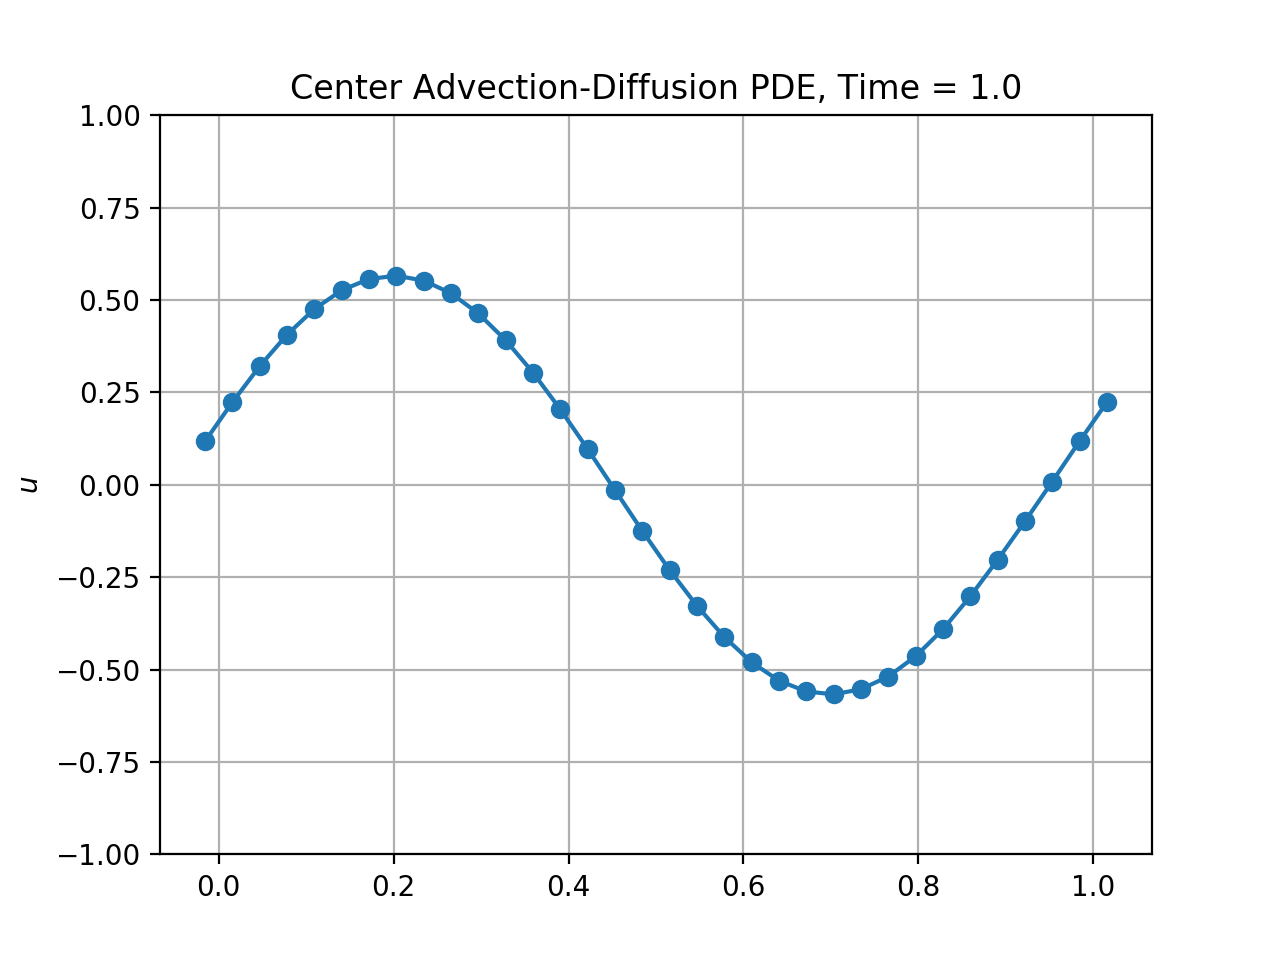
\includegraphics[width=0.7\linewidth]{./PDE/figures/plotsforh/result_advection_diffusion_32_center_h.png}
		\caption{The solution to the advection-diffusion PDE using the centered discretization method.}
		\label{fig:addiff}
	\end{figure}
	
	\end{enumerate}



\section{Conclusion}

As we can see from the previous results, the Fortran implementations solve the PDEs succesfully. In addition, the Fortran code collects the \texttt{pde.init} file and reads the runtime parameters, then collects results and writes text files. The Python script then plots the results. Although I obtain correct solutions, I believe there is some parts of the code that can be optimized or better organized. The biggest issue was automating when to output the text files for the correct time.
	









\end{document}